\section{The Bradley-Terry-Luce Model for Paired Comparisons}\label{sec:logist-btl}
The basic methodology of logistic regression finds application in
a surprising variety of applications
\citep{Strauss:92}.
One example is a model for paired comparisons data proposed by
\citet{BradleyTerry:52}, and by \citet{Luce:59} in a more general context.
In paired comparisons, $K$ objects are compared in a pairwise manner
and the goal is to determine scale values and a ranking of these objects.
For example, a market researcher might wish to construct a preference ranking for
soft drinks among consumers.  In other contexts, the objects might be
teams or players in a sports league, or sounds of varying intensity
or frequency to be judged in a psychophysical experiment.

The Bradley-Terry-Luce (BTL) model assumes that, for each object there is
a parameter, $\theta_i$, such that the probability of the event $(i > j)$
that object $i$
is preferred to object $j$ is
\begin{equation}\label{eq:btl1}
\Pr ( i > j ) = \frac{\theta_i}{\theta_i + \theta_j}
\period
\end{equation}
Luce's model is more general, and $\theta_i$ is interpreted as
the probability that object $i$ is ranked first within \emph{any} subset
of objects.
The BTL model \eqref{eq:btl1} may be cast as a logit model with parameters
$\beta_i,= \log \theta_i$ as follows.
Substituting $\theta_i = \exp (\beta_i)$ in \eqref{eq:btl1} gives,
\begin{equation}\label{eq:btl2}
\Pr ( i > j ) = \frac{\exp(\beta_i)}{\exp(\beta_i) + \exp(\beta_j)}
     = \frac{1}{1 + \exp(\beta_i / \beta_j)}
	  \period
\end{equation}
But \eqref{eq:btl2} is just the inverse logit of $\theta_i/\theta_j$. Hence,
\begin{eqnarray}
\logit [ \Pr (i>j)] = \log \left( \frac{\Pr (i>j)}{\Pr (j>i)} \right)
    & = & \beta_i - \beta_j  \label{eq:btl3} \\
    & = & \vec{x}\trans \vec{\beta} \nonumber
\end{eqnarray}
where, $\vec{\beta} = ( \beta_1, \dots , \beta_K)\trans$ and
$\vec{x} = \{x_k\}$ is a vector with
$x_k = 1$ if $k=i$, $x_k = -1$ if $k=j$, and 0 otherwise.
Thus, model \eqref{eq:btl3} is a logit model with no intercept,
and with a $K (K-1)/2 \times K$ matrix $\mat{X}$ of explanatory
variables whose rows give the items compared in each
paired comparison.  For $K=4$ objects, for example, the $\mat{X}$ matrix is
\begin{equation*}
 \mat{X} = \left[
  \begin{array}{rrrr}
  1 & -1 & 0 & 0 \\
  1 & 0 & -1 & 0 \\
  1 & 0 & 0 & -1 \\
  0 & 1 & -1 & 0 \\
  0 & 1 & 0 & -1 \\
  0 & 0 & 1 & -1 \\
  \end{array}
 \right]
 \period
\end{equation*}

The model assumes that all comparisons are independent.  In particular,
when items are rated by different judges,  the ratings of different
pairs by the same judge must also be independent, and all judges are
assumed homogeneous.
More general versions of the BTL model, allowing subject-specific
covariates, are described by \citet{Dittrich-etal:1998}.

\begin{Example}[winloss]{1987 baseball standings}
\tabref{tab:winloss} (from \citet[p. 372]{Agresti:90}) shows the
final results from the 1987 baseball season for the teams in the Eastern Division
of the American League.
Each team played every other team a total of $n_{ij} = 13$ times,
so (assuming that the outcome of each game is independent)
we may regard the values in the lower triangle
as binomial observations, $\Bin( \pi_{ij}, 13 )$.
\begin{table}[htb]
 \caption{1987 American League Baseball Results}\label{tab:winloss}
 \begin{center}
 \begin{tabular}{l| rrrrrrr}
 \hline
 Winning & \multicolumn{7}{c}{Losing Team} \\ \cline{2-8}
 Team    & Mil & Det & Tor & NY & Bos & Cle & Bal \\
 \hline
Milwaukee & $-$ &  7  &  9  &  7  &  7  &  9  & 11 \\ 
Detroit   &  6  & $-$ &  7  &  5  & 11  &  9  &  9 \\ 
Toronto   &  4  & 6   & $-$ &  7  &  7  &  8  & 12 \\ 
New York  &  6  & 8   &  6  & $-$ &  6  &  7  & 10 \\ 
Boston    &  6  & 2   &  6  &  7  & $-$ &  7  & 12 \\ 
Cleveland &  4  & 4   &  5  &  6  &  6  & $-$ &  6 \\ 
Baltimore &  2  & 4   &  1  &  3  &  1  &  7  & $-$ \\ 
 \hline
 \end{tabular}
 \end{center}
\end{table}


We concentrate here on fitting the BTL model and graphical displays of
the scale values and model diagnostics.
A similar example, without graphs, is given in
\emph{Logistic Regression Examples Using the SAS System}, Example 19.

The first \Dstp\ below reads the complete data from \tabref{tab:winloss}.
In a second step, variables in the array \pname{X} are created, corresponding
to the model matrix in \eqref{eq:btl3}.
The resulting \Dset, \pname{winloss2} is shown in \outref{out:btl2.1}.
%% input: /Users/friendly/sasuser/catdata/btl2.sas
%% last modified: 29-Jul-99  9:21
\begin{listing}
title 'Bradley-Terry-Luce Model, 1987 American League, East';
data winloss;
  input t1-t7;
  games=13;
datalines;
  .  7  9  7  7  9 11
  6  .  7  5 11  9  9
  4  6  .  7  7  8 12
  6  8  6  .  6  7 10
  6  2  6  7  .  7 12
  4  4  5  6  6  .  6
  2  4  1  3  1  7  .
;
data winloss2;
   retain i 0 ;
   array team\{*\} t1-t7;
   array x\{*\} milwauke detroit toronto new_york boston clevelan baltimor;
   retain milwauke detroit toronto new_york boston clevelan baltimor 0;
   set winloss;
   names='Milwaukee Detroit Toronto New_York Boston Cleveland Baltimore';
   length winner loser $9;
   i+1;
   do j=1 to dim(team);
      if team\{j\} ne . then do;
         count=team\{j\};
         x\{i\}=1;
         x\{j\}=-1;
         winner = scan(names,i);
         loser  = scan(names,j);
         if i < j then output;
         x\{i\}=0;
         x\{j\}=0;
      end;
   end;
   drop i j t1-t7 names;
\end{listing}


\begin{Output}[!htb]
\caption{Win-loss data, set up for fitting BTL model with \PROC{LOGISTIC}}\label{out:btl2.1}
\small
\verbatiminput{ch6/out/btl2.1}
\end{Output}
The BTL model is fit using the \PROC{LOGISTIC} step below.
The options \pname{OUTEST} and \pname{COVOUT} create an \ODS\
containing the estimated $\beta_i$ parameters and their
variance-covariance matrix.
A second \ODS\ containing fitted probabilities and model diagnostic
measures is created with the \stmt{OUTPUT}{LOGISTIC}.
The parameters and their standard errors are shown in \outref{out:btl2.2}.
Thus, according to the BTL model \eqref{eq:btl1},
the predicted probability that Toronto beats Cleveland would be
$\exp(1.294)/(\exp(1.294) + \exp(0.684)) = 0.648$.
The squared standard errors are contained along the diagonal of the
variance-covariance matrix in the \pname{PARM1} \Dset.
A small \IML\ step is used to extract the parameter estimates and
standard errors.
%% input: /users/faculty/friendly/sasuser/catdata/btl2.sas
%% last modified: 15-Sep-98 11:29
\begin{listing}
proc logistic data=winloss2 nosimple out=parm1 covout;
  model count/games=milwauke detroit toronto new_york
                    boston clevelan baltimor / noint;
  output out=fit prob=prob resdev=resdev c=c;
run;

*-- Extract parameters and standard errors;
proc iml;
   use parm1;
   read all var \{_name_\} into name where(_type_='COV');
   read all var \{milwauke detroit toronto new_york
                 boston clevelan baltimor\} into parm where(_type_='PARMS');
   read all var \{milwauke detroit toronto new_york
                 boston clevelan baltimor\} into cov where(_type_='COV');

   stderr = exp(sqrt(vecdiag(cov)));
   parm = exp(t(parm));
   create parms var \{name parm stderr\};
   append var \{name parm stderr\};

proc rank data=parms out=parms descending;
   var parm;
   ranks rank;
   label parm='Scale Value'
      rank='Team Rank';
\end{listing}

\begin{Output}[htb]
\caption{Win-loss data, \PROC{LOGISTIC} output}\label{out:btl2.2}
\small
\verbatiminput{ch6/out/btl2.2}
\end{Output}

%% one figure
\begin{figure}[!htb]
  \centering
  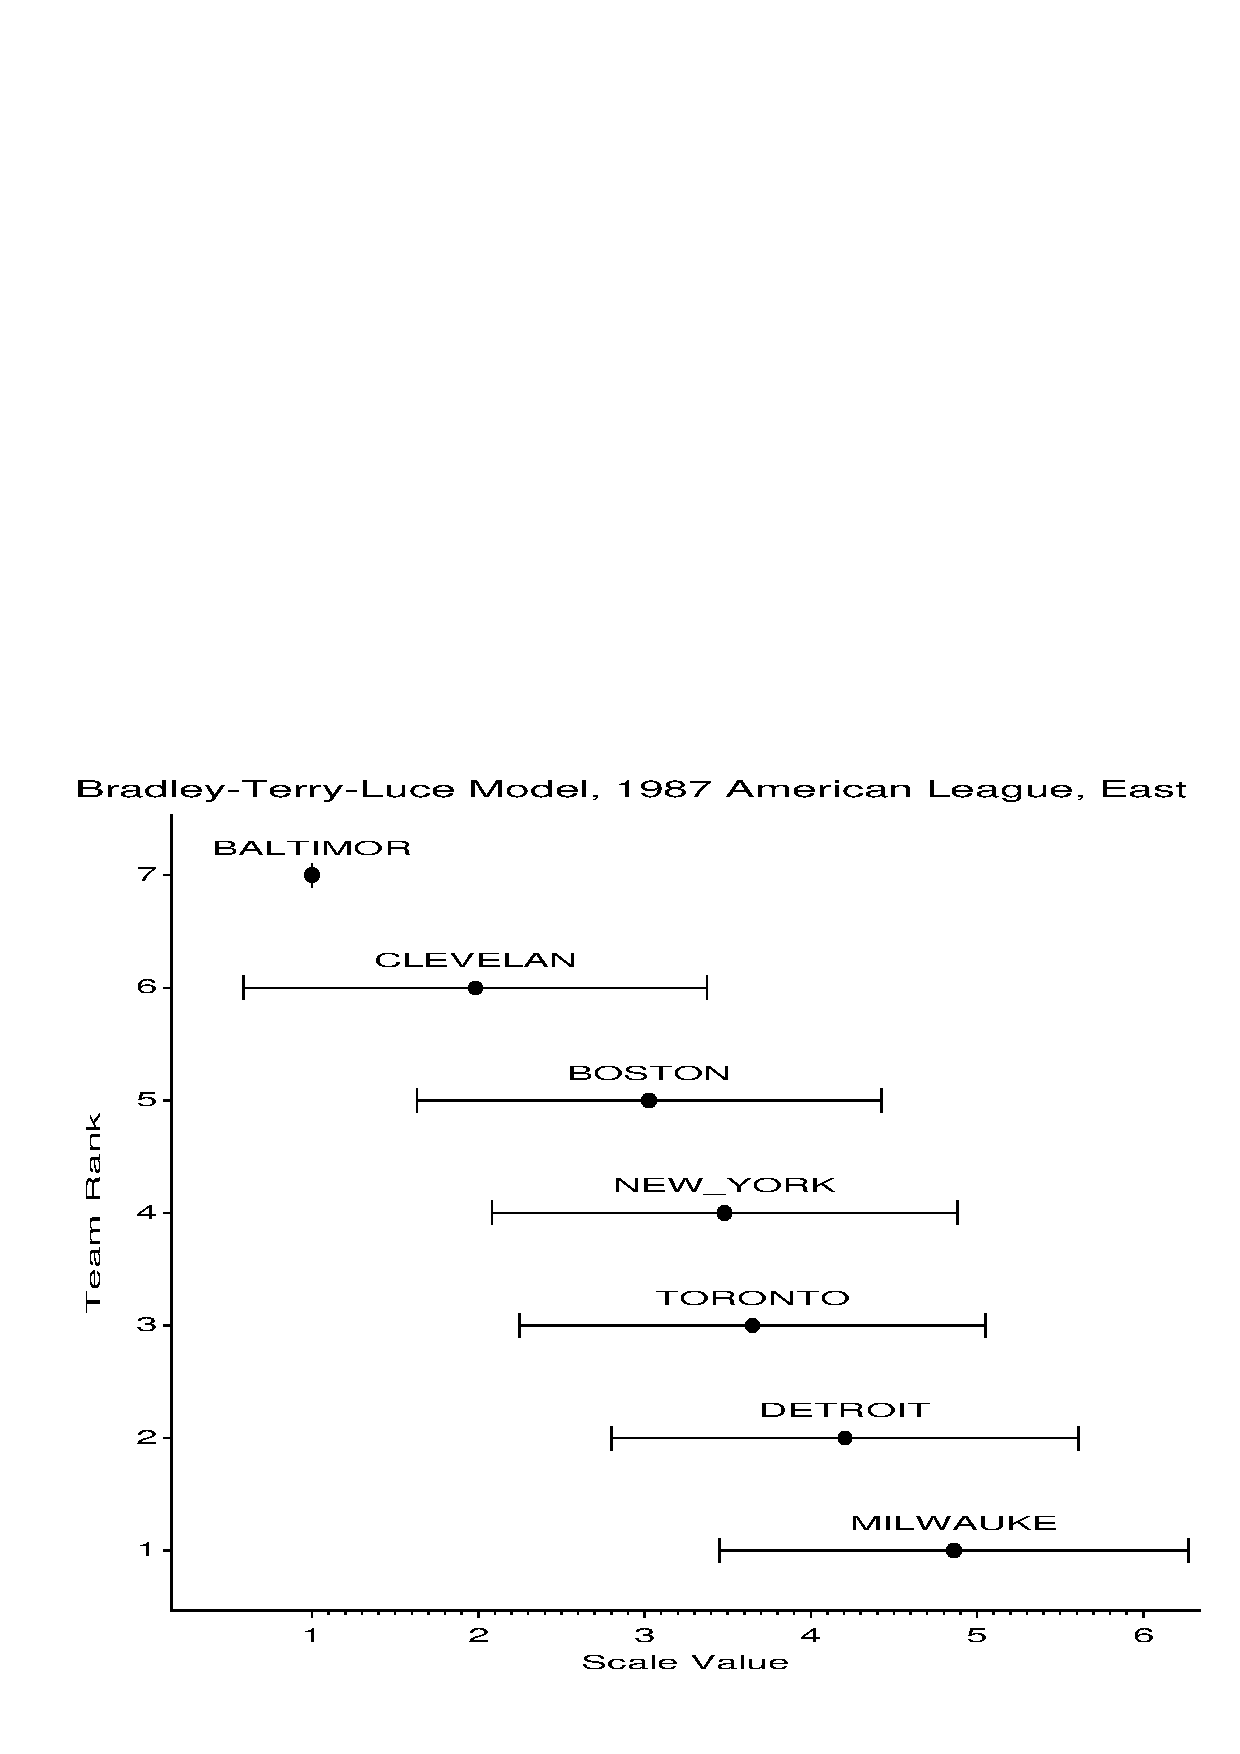
\includegraphics[scale=.6]{ch6/fig/btl21}
  \caption{Scale values and standard errors for 1987 baseball data}%
  \label{fig:btl21}
\end{figure}
The plot of scale values and standard errors shown in \figref{fig:btl21}
is produced by the first \PROC{GPLOT} step below.
The \macro{BARS} constructs the \ADS\ to draw the standard error bars,
and the \macro{LABEL} produces the team label annotations.
%% input: /users/faculty/friendly/sasuser/catdata/btl2.sas
%% last modified: 15-Sep-98 11:29
\begin{listing}
%bars(data=parms, var=parm, class=rank, barlen=stderr, baxis=x, barwidth=.1);
%label(data=parms, x=parm, y=rank, text=name, pos=2, yoff=.1, out=_lab_);
data _bars_;
   set _bars_ _lab_;

proc gplot data=parms;
   plot rank * parm / 
      anno=_bars_ vaxis=axis1 haxis=axis2 vm=0;
   symbol v=dot color=black h=1.6;
   axis1 label=(a=90) offset=(5);
    axis2 order=(1 to 6) offset=(10,4);
run; quit;

%label(data=fit, x=prob, y=resdev, out=_lab_,
   subset=%str(abs(resdev)>.9),
   text = %str(substr(winner,1,3) || '>' || substr(loser,1,3)));
title;
proc gplot data=fit;
   bubble resdev * prob = c /
      anno=_lab_ bsize=20 bcolor=gray80 vaxis=axis1 vm=1;
   axis1 label=(a=90);
   label prob = 'Estimated Winning Probability';
\end{listing}


%% one figure
\begin{figure}[htb]
  \centering
  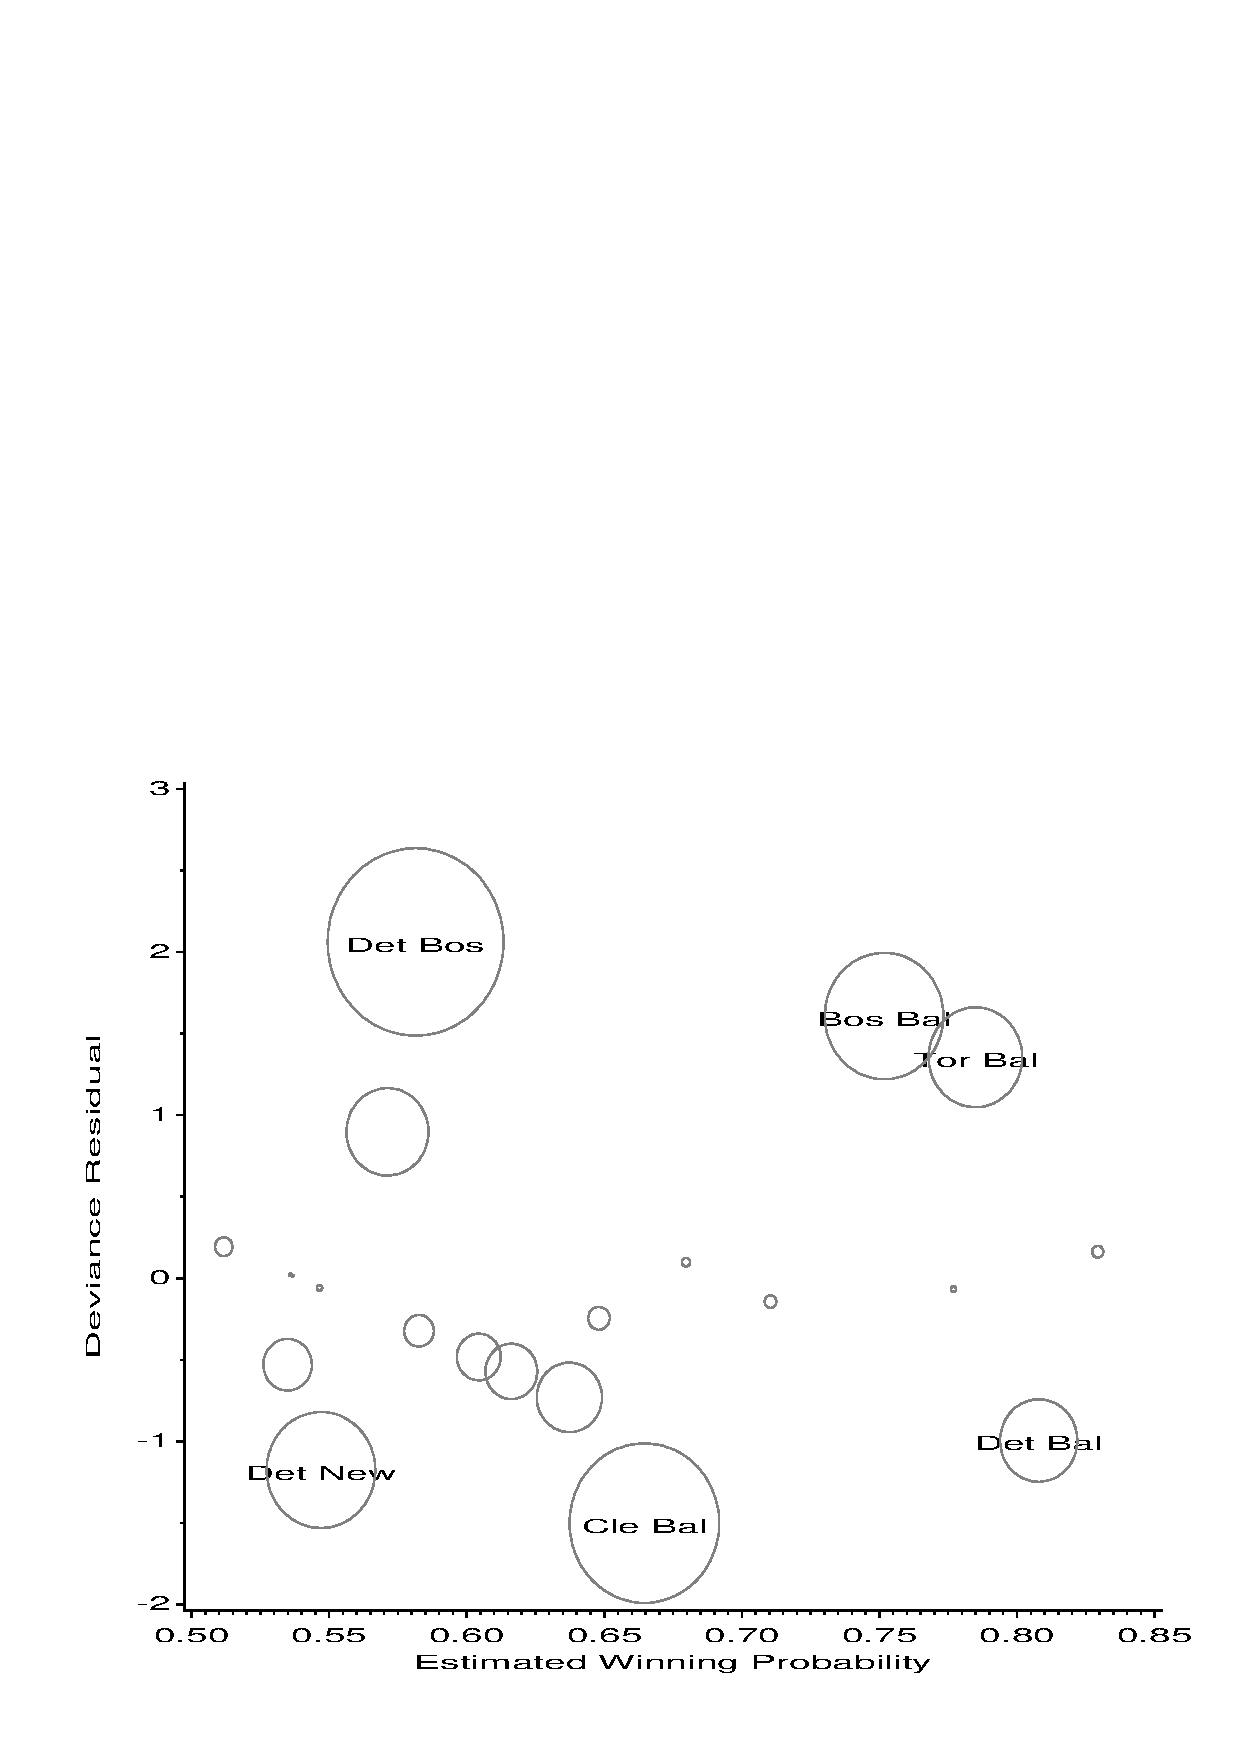
\includegraphics[scale=.6]{ch6/fig/btl22}
  \caption{Diagnostic plot for 1987 baseball data}%
  \label{fig:btl22}
\end{figure}
The diagnostic plot shown in \figref{fig:btl22} plots the deviance residual
against predicted probabilities.  The bubble size is proportional to Cook's
distance, $C_i$.  Only one observation has a residual (slightly) greater than 2,
and no $C_i$ are excessive, so the BTL model seems to provide a reasonable
fit.
\end{Example}
